\section{Experimental Evaluation}
\label{sec:experiments}

We have evaluated MBFQ extensively. Due to lack of space, we only present
selected microbenchmarks in this paper. Our microbenchmarking testbed consists
of two Dell PowerEdge R410 servers.  Both servers have four 2.26GHz cores, with
hyper-threading enabled, which gives it 8 logical processors.  Each machine has
8GB of RAM and 10G NIC.  Both machines run a flavor of Windows Server OS with
Hyper-V enabled for network virtualization. This configuration emulates our
common use case: VMs communicating with other VMs in the same data
center.~\footnote{In modern data centers, most traffic is
intra-DC~\cite{fb,kandula09}.} 

\subsection{Picking a Timer Period for Measurement}
{\bf Question:}  The macrosheduler runs every $T$ time units. What is the right
value of $T$?

{\bf Motivation:}  As discussed earlier, it can take up to three iterations (thus
$3*T$) for the macroscheduler to allocate a VM with its minimum
guaranteed bandwidth. Therefore, we don't want $T$ to be too large. On the other hand,
recall that we measure send rate over the same time period. If $T$ is too small,
the measured send rate of the VM ($SR$) may be inaccurate. The primary source of
inaccuracy is inherent burstiness of TCP. To estimate the inaccuracy for
various values of $T$, we carried out the following experiment.

{\bf Experiment}: A single VM hosted on one of the servers sends data to
an external server using TCP. In all, 32 TCP connections were used. The application 
generated data at 7.2Gbps. All rate
allocation functionality of MBFQ was disabled, only the measurement code was
active.  We logged the measured send rate ($SR$) over 100 intervals.  We
repeated experiment for values of $T$ ranging from 15ms to 1000ms.
Figure~\ref{variation} shows the standard deviation as a function of $T$.  

\begin{figure}
\centering
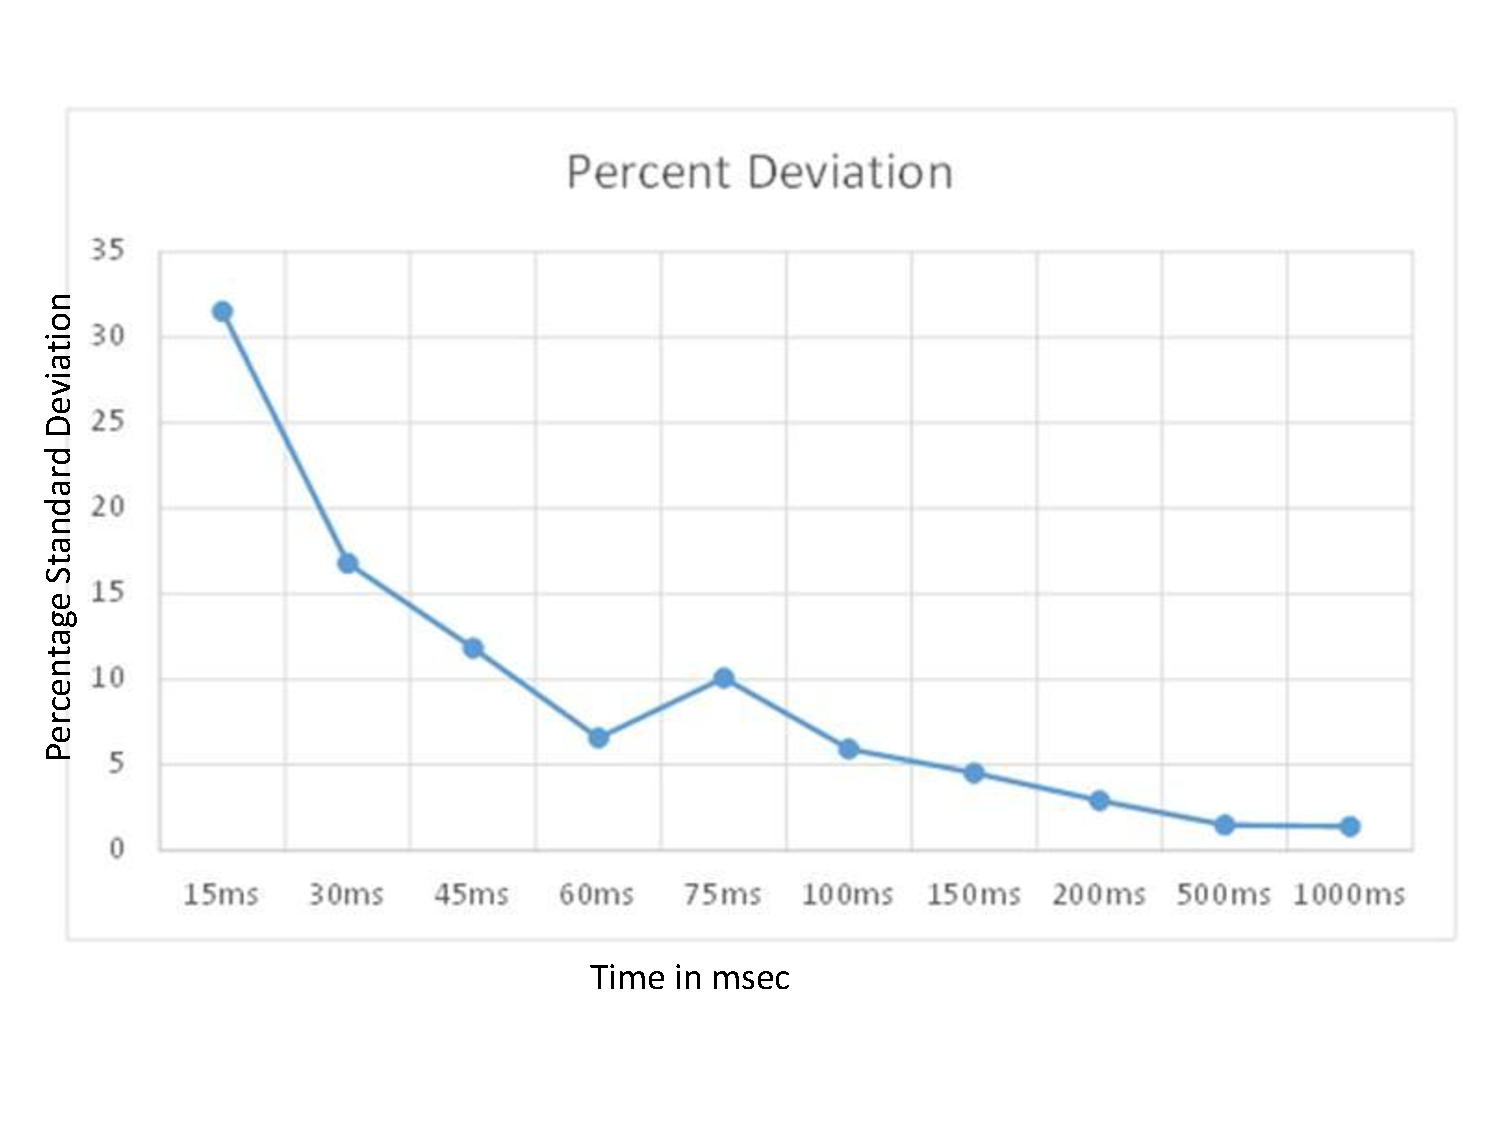
\includegraphics[width=0.7\columnwidth, trim=60pt 20mm 0pt 8mm]{figures/variation}
\caption{Impact of $T$ on variance in $SR$}
\label{variation}
\vspace{-3mm}
\end{figure}

{\bf Discussion:} A value of $T$ between 60 - 100ms reduces standard deviation
of $SR$ to $5\%$.  Larger $T$ will lead to further reduction, but decrease is
small.

While a 100ms initial response time is not suitable for some latency-sensitive applications,
many applications that we tested, including video streaming and file transfers, can tolerate
this delay. Latency-sensitive applications can use hardware-assisted QoS such as 802.1p
to isolate their traffic from the general VM traffic.  Alternatively, an implementation of MBFQ
could have a combination of static and dynamic bandwidth allocations where latency-sensitive
VMs are assigned static queues, and other VMs dynamically share the remaining bandwidth.

\subsection{Bandwidth Ramp Up and Ramp Down}
\label{sec:fairshare}
{\bf Question:} A VM may have to wait for up to three macroscheduler intervals to reach its
minimum guaranteed bandwidth. Also, we wait for up to 500 milliseconds before we
reclaim bandwidth from a VM that is not fully using the allocated bandwidth. Are
these time intervals appropriate?

{\bf Motivation:}  While the allocated bandwidth to VM ramps up to the minimum
guaranteed bandwidth in three intervals, the VM may not be able to ramp up as
quickly, due to limitations of the TCP congestion control. Furthermore, waiting
for 500 milliseconds before reclaiming the bandwidth may lead to
under-utilization of the link.

{\bf Experiment:}  A test machine hosts 4 VMs with the following
minimum bandwidth guarantees: VM1: 100Mbps (relative weight: 1), VM2: 100Mbps
(relative weight: 1), VM3: 1Gbps (relative weight: 10), VM4: 3Gbps (relative
weight: 30). Each of the VMs sends traffic to an external machine ("client
machine") over the shared 10G external physical NIC.  The link is configured to
share 9.5Gbps among the VMs.  Each VM is always 
backlogged and tries to send data as fast as it can.

Figure~\ref{fairsharing}  shows the transmit bandwidth for each VM, and the
total transmit bandwidth in several phases. 

\begin{figure}[h]
\centering
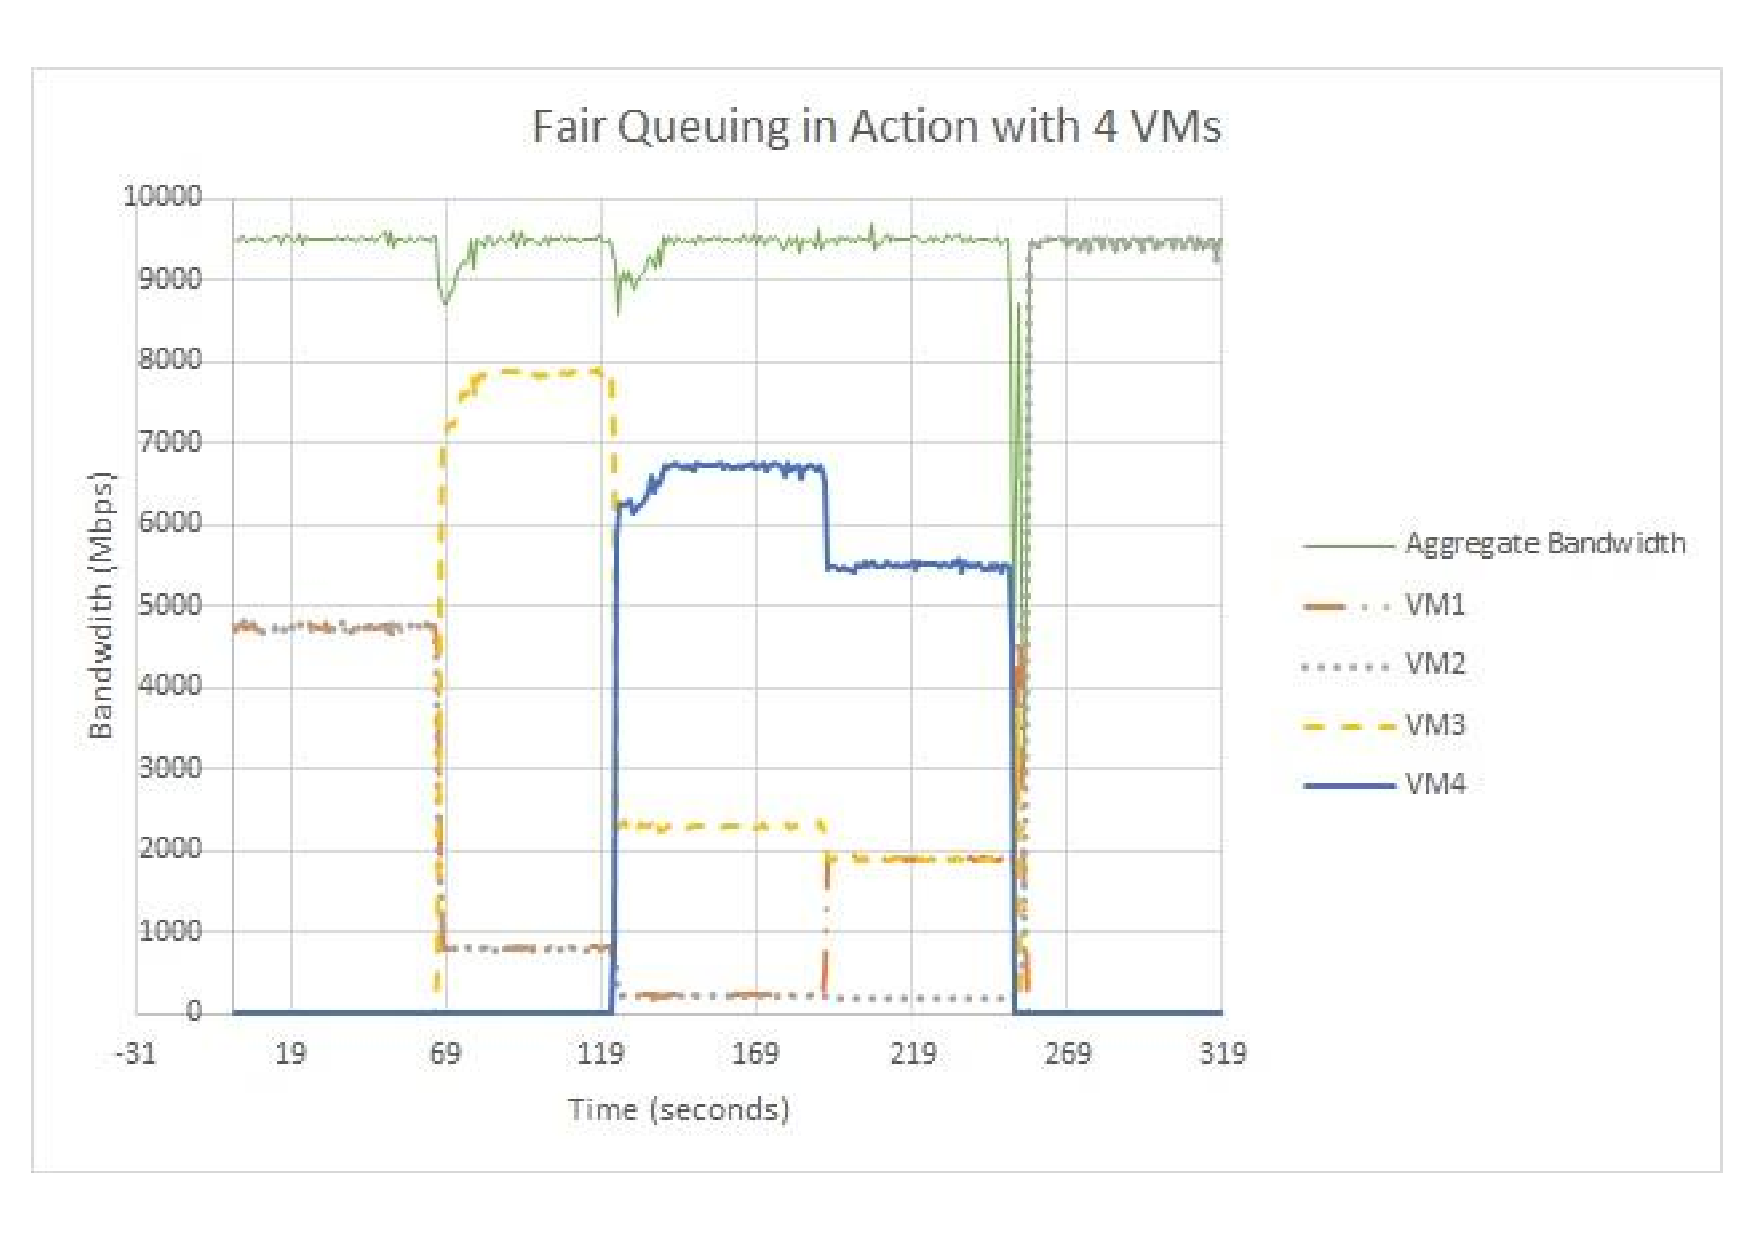
\includegraphics[width=0.8\columnwidth,trim=60pt 20mm 0pt 8mm]{figures/fairsharing}
\caption{Ramp up and ramp down test}
\label{fairsharing}
\vspace{-3mm}
\end{figure}

{\bf Phase 1:}  At time 0, only VM1 and VM2 are active. As expected, they share
the bandwidth equally, with each getting 4.75Gbps.

{\bf Phase 2:} At time 69, VM3 starts transmitting. MBFQ quickly
throttles VM1 and VM2 to 792Mbps each, while VM3 is allowed to use 7.92Gbps. 

{\bf  Phase 3:} At time 119, VM4 starts transmitting. The four VMs now
get their weighted fair share: VM1 and VM2 get 226Mbps, VM3
gets 2.26Gbps and VM4 gets 6.79Gbps. 

{\bf  Phase 4:} At time 189, we change the min bandwidth guarantee of VM1 from
100Mbps to 1Gbps. VM1 and VM3 now both transmit at the same rate, and the rates
of VM2, VM3, and VM4 were reduced to accommodate the increase in VM1's rate.

{\bf Phase 5:} At time 249, VM1, VM3, and VM4 stop sending. VM2
ramps up to consume the full link bandwidth.

{\bf Discussion:} We see that while MBFQ generally performs well, there are dips
in link utilization at times 69 and 119 as VMs ramp up. The dips in the aggregate
bandwidth at the beginning of phases 3
and 4 are due to our desire to allow a VM to quickly attain minimum
guaranteed bandwidth. As VM3 and VM4 are ramping up, the algorithm detects that
the VMs requests for additional bandwidth in several consecutive iterations.
Therefore, in order to quickly provide the VMs their subscribed bandwidth, after
three consecutive iterations of additional bandwidth requests, the algorithm
allocates the full fair share of bandwidth to the VM. However, even after
    the bandwidth is allocated, the VMs could take some time to consume all allocated
bandwidth, due to
TCP artifacts. Thus, the dip represents a trade-off between how fast the
algorithm should grant a VM its fair share versus how cautious it should be in
allocating the VM bandwidth that it might not be ready to consume (and thus risk
being non-work conserving). A more extreme dip is seen at the
beginning of phase 5, we shall discuss that in Section \ref{reclaimbw}.

\subsection{Can we ramp up any faster?}

{\bf Question:}  Is the ramp up delay shown in Figure~\ref{fairsharing} for VM3
at 69 seconds caused by our algorithm or it due to the VM itself (e.g., its TCP
behavior)?

{\bf Motivation:} The previous experiment suggests the algorithm may be too slow
in allocating bandwidth to a newly active VM.  

{\bf Experiment:} We measure bandwidth ramp up in two scenarios.  First, we
measure a  ``standalone'' scenario where VM3 is the only VM transmitting (i.e. the link
was idle before VM3 started sending).  Second, we measure a  ``sharing'' scenario
in which the link was fully utilized before VM3 started sending. When VM3 starts
sending, MBFQ performs bandwidth allocation to give VM3 its fair share.

\begin{figure}[h]
\centering
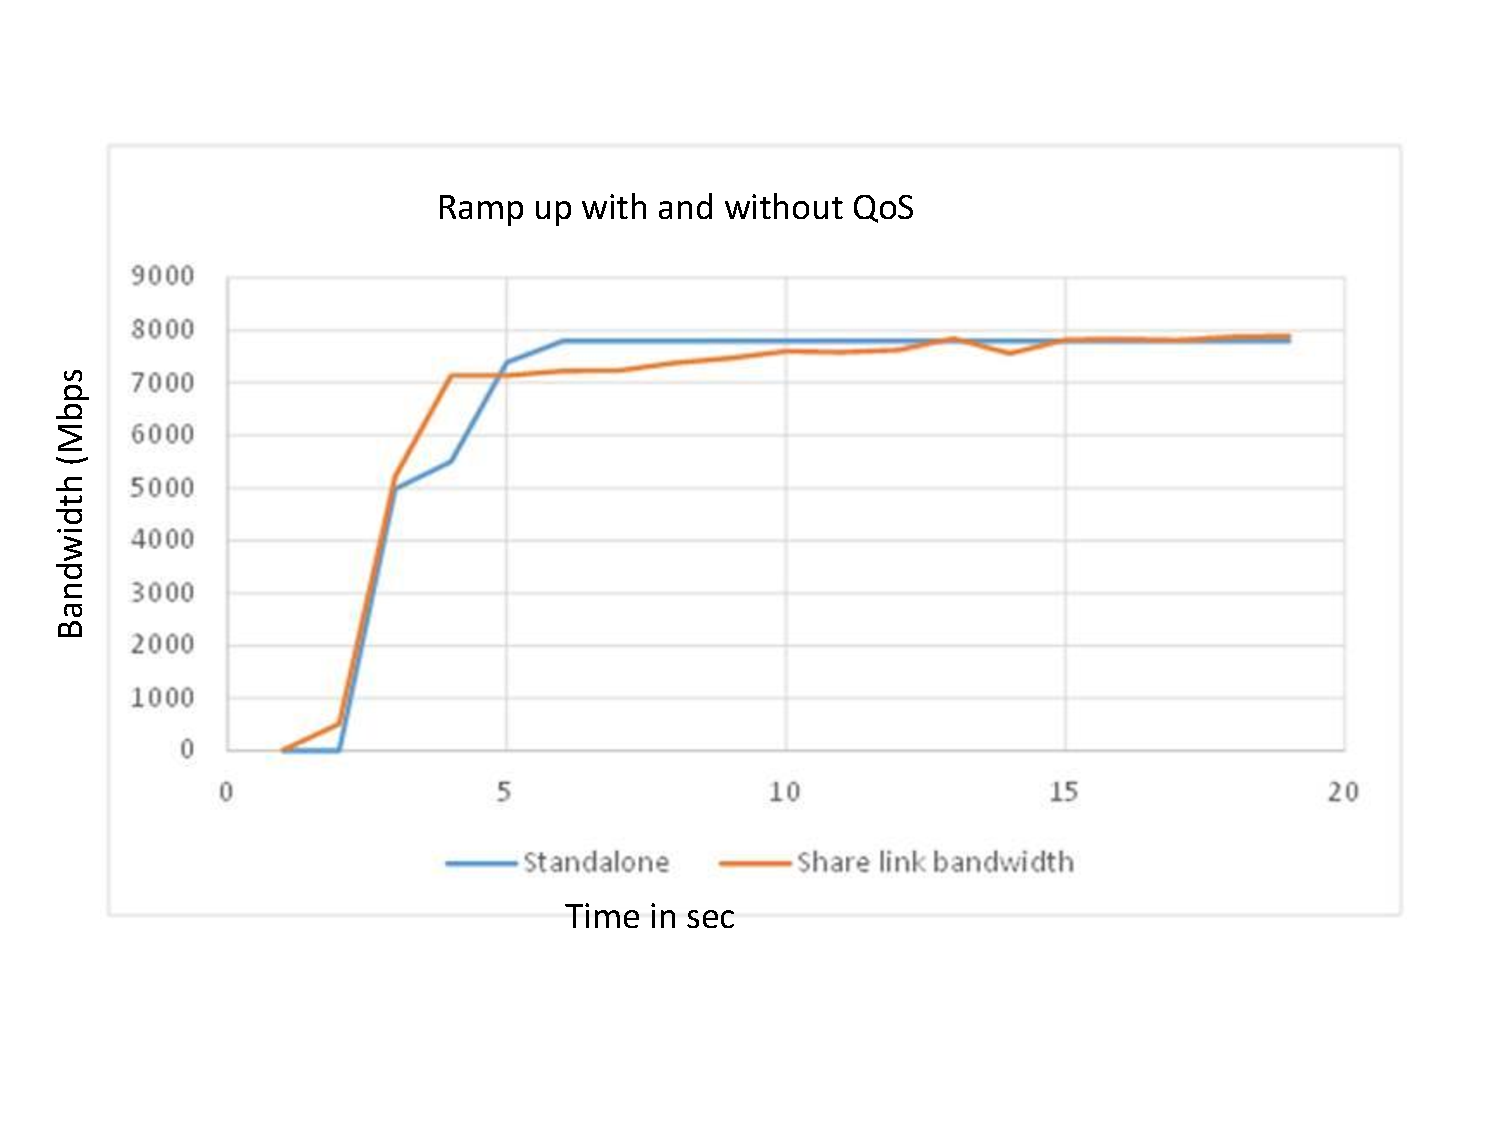
\includegraphics[width=0.6\columnwidth,trim=60pt 40mm 0pt 8mm]{figures/rampupcomparison}
\caption{TCP and MBFQ ramp up}
\label{rampupcomparison}
\vspace{-3mm}
\end{figure}

{\bf Discussion:} As seen in Figure~\ref{rampupcomparison}, it takes about the
same amount of time in both scenarios for VM3 to achieve most of its bandwidth
(up to 7Gbps). However, it takes an additional 15s for VM3 to reach its steady
state  in the "Share link bandwidth" scenario. However, in the sharing scenario,
the VM is transmitting on top of a NIC that is already fully utilized.
But in the standalone case, the VM is transmitting on top of an idle NIC. 

{\bf Conclusion:} It is probably not worthwhile 
to ramp up faster because TCP may not be able to fully utilize the extra
bandwidth quickly.

\subsection{How fast should we reclaim bandwidth?}
\label{reclaimbw}
{\bf Question:}  The faster we reclaim bandwidth the
faster we redistribute it other needy VMs who can use it. How large should the
reclaim period $T$ be?

{\bf Motivation:} 
We see a large dip in the utilization at the beginning of Phase 5 in
Figure~\ref{fairsharing} when VM1, VM3, VM4 stop sending.  In addition to the
TCP ramp-up time of VM2, the dip is also partly due to another parameter in the
algorithm where we configure the algorithm to wait for 500 milliseconds before
reclaiming residual bandwidth.  Unfortunately, this is a tradeoff.  The faster we
reclaim, the more likely the algorithm is to spuriously reclaim bandwidth from a
paid customer VM which has short term bursts.

{\bf Experiment:} We measure the impact of different reclaim timer values on the
throughput of a large file transfer operation in a VM.  We have VM1 host a large
file that is being copied to a remote machine, while VM2, VM3, VM4 send background CBR traffic
to fill up the idle link.  The file transfer application on
VM1 uses about 800Mbps, and the rest of the link bandwidth is distributed among
VM2, VM3, VM4.  We change the wait time parameter from No Wait (at every
macroshedular iteration, bandwidth is immediately reclaimed if VM1 is
sending less than 85\% of its allocated rate) to 1000ms wait (bandwidth is not
reclaimed unless the VM has been sending less than 85\% of its allocated rate in
the last 1000ms)

\begin{figure}[h]
\centering
\subfigure[Reclaim timer of 500 msec and 1000 msec]
{
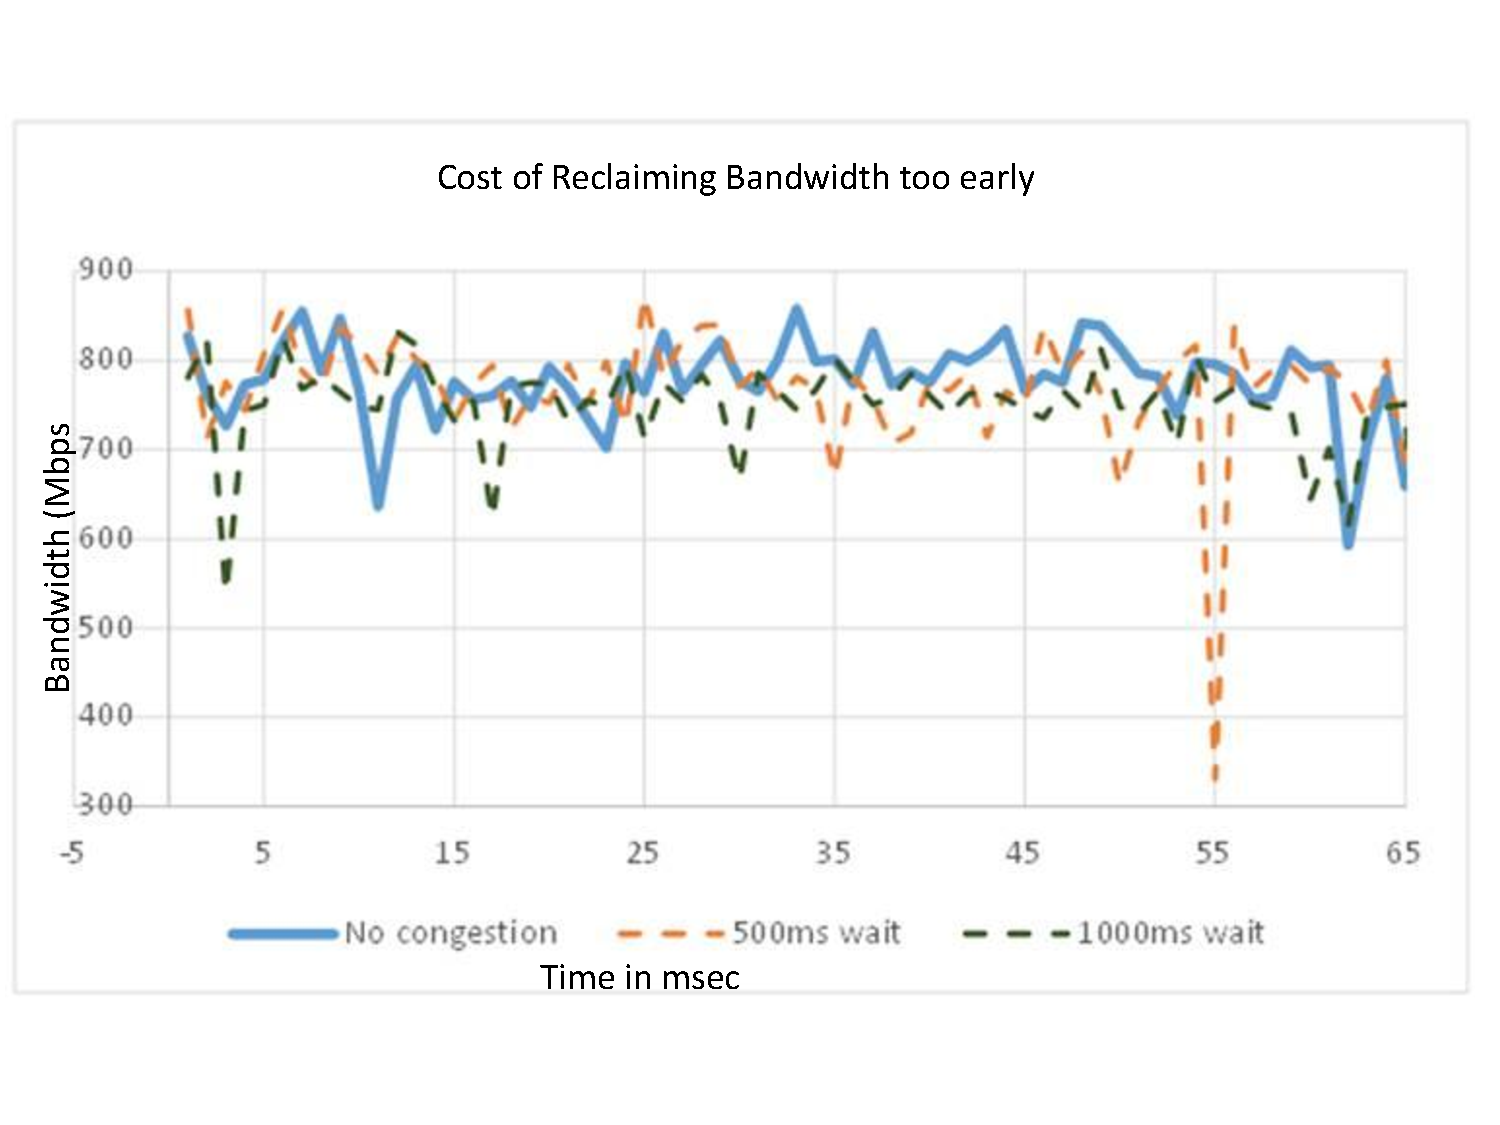
\includegraphics[width=0.7\columnwidth,trim=60pt 20mm 0pt 8mm]{figures/rampdowntime1}
\label{rampdowntime1}
}
\subfigure[Reclaim timer of 0 msec and 200 msec.]
{
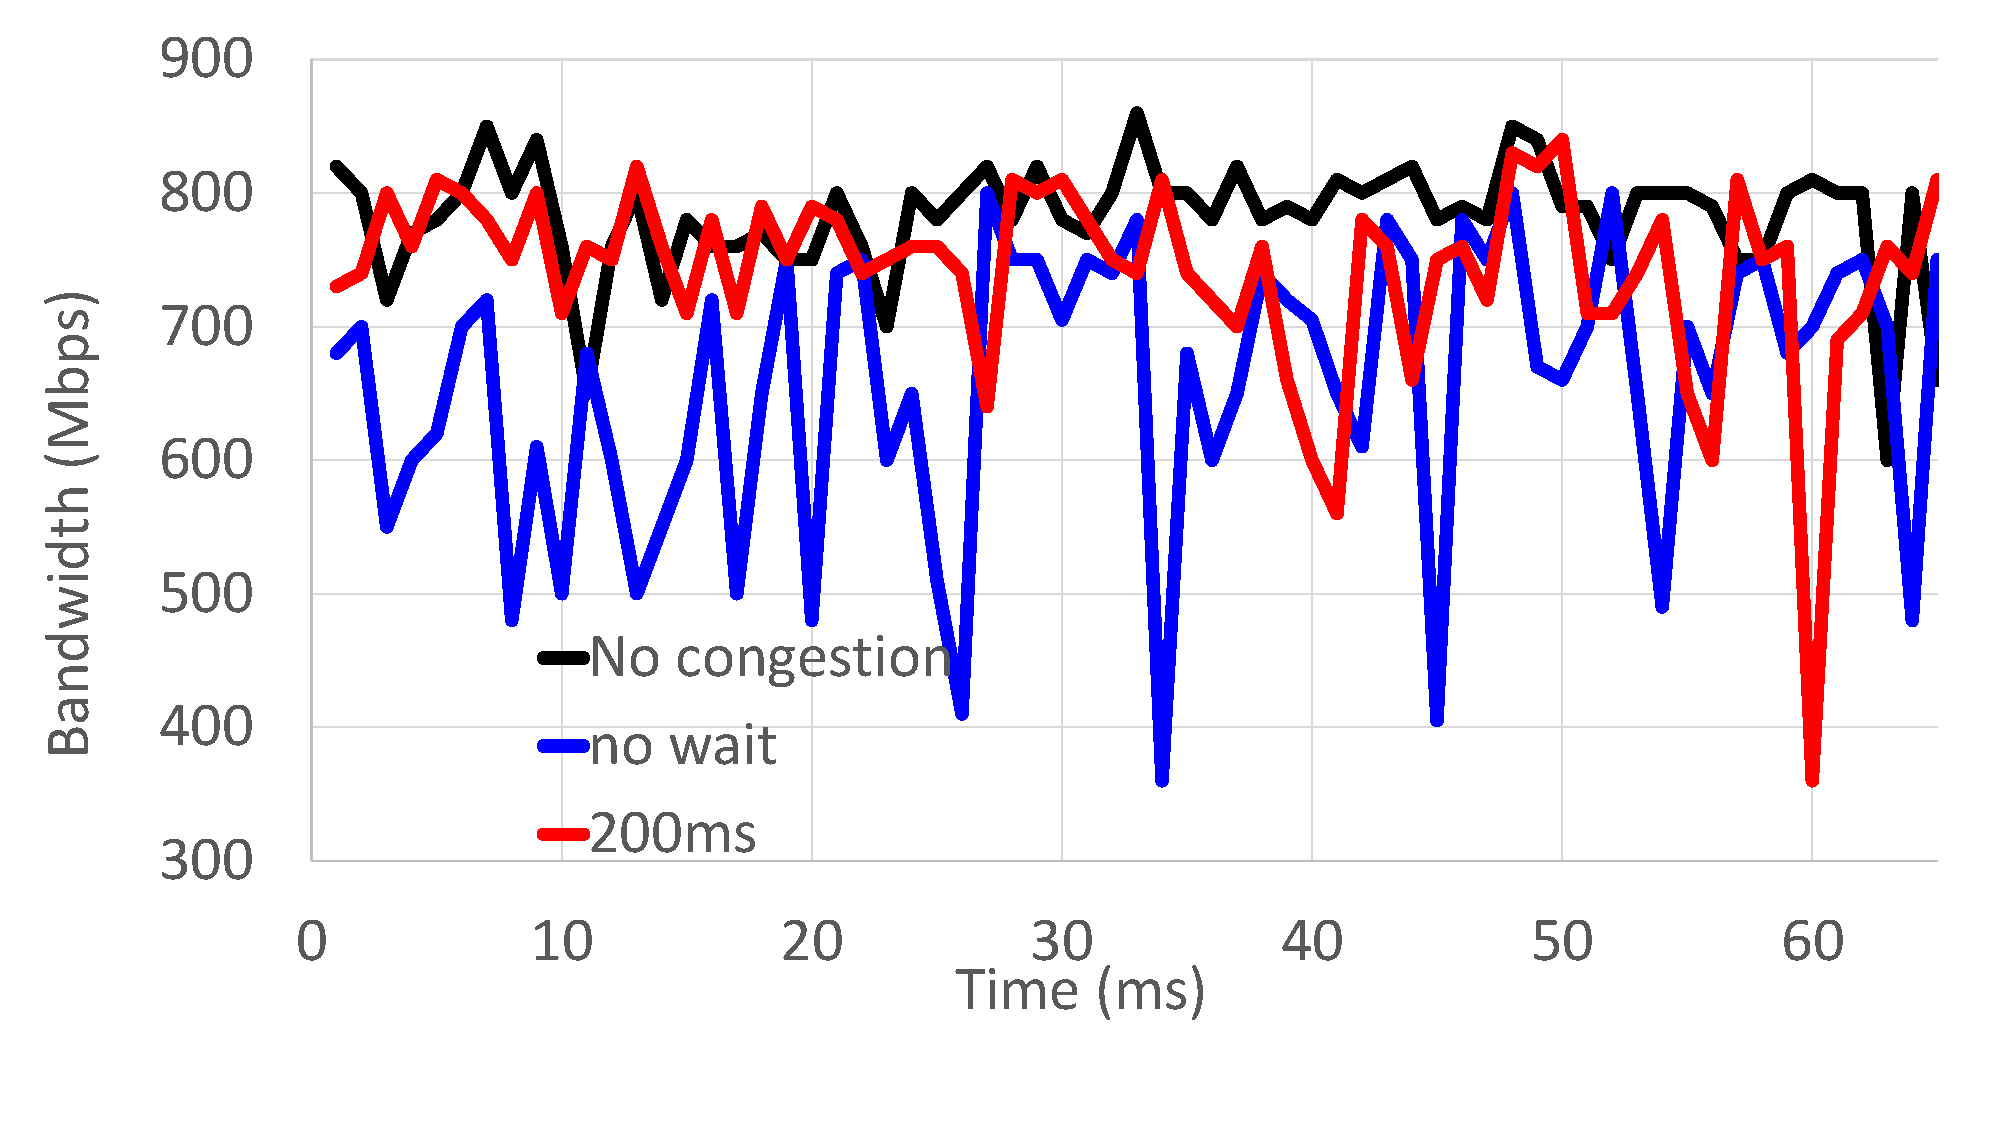
\includegraphics[width=0.7\columnwidth,trim=60pt 20mm 0pt 8mm]{figures/rampdowntime2}
\label{rampdowntime2}
}
\vspace{-1em}
\caption{Impact of reclaim timer}
\vspace{-1em}
\label{fig:reclaim}
\end{figure}

Figure~\ref{rampdowntime1} shows that the bandwidth stays roughly the same with
MBFQ and without MBFQ with a reclaim timer of 500 or 1000 msec. On the other
hand, Figure~\ref{rampdowntime2} shows that with instantaneous reclaiming
(reclaim timer of 0) the bandwidth allocated to the VM is significantly affected
and its noticeable even at a reclaim timer of 200 msec.

{\bf Conclusion:}  A reclaim timer of 500 milliseconds was chosen as a 
compromise. 

\subsection{CPU Utilization}
\label{sec:utilization}

We measure the CPU overhead of MBFQ for the setup in Section~\ref{sec:fairshare}
by comparing the CPU utilization of that setup to the CPU utilization of a base scenario
without MBFQ.  

For the base scenario, we assign static rate limits to VM1, VM2, VM3, and VM4
with 226Mbps, 226Mbps, 2.26Gbps, and 6.79Gbps respectively.  These are the rates
that MBFQ dynamically distributes  to the VMs when all VMs are active.

With all VMs active, the CPU utilization of the base scenario is 22.74\%, and CPU utilization
with MBFQ is 23.22\%. This shows that MBFQ has minimum CPU overhead.
